\documentclass[twoside]{book}

% Packages required by doxygen
\usepackage{calc}
\usepackage{doxygen}
\usepackage{graphicx}
\usepackage[utf8]{inputenc}
\usepackage{makeidx}
\usepackage{multicol}
\usepackage{multirow}
\usepackage{textcomp}
\usepackage[table]{xcolor}

% Font selection
\usepackage[T1]{fontenc}
\usepackage{mathptmx}
\usepackage[scaled=.90]{helvet}
\usepackage{courier}
\usepackage{amssymb}
\usepackage{sectsty}
\renewcommand{\familydefault}{\sfdefault}
\allsectionsfont{%
  \fontseries{bc}\selectfont%
  \color{darkgray}%
}
\renewcommand{\DoxyLabelFont}{%
  \fontseries{bc}\selectfont%
  \color{darkgray}%
}

% Page & text layout
\usepackage{geometry}
\geometry{%
  a4paper,%
  top=2.5cm,%
  bottom=2.5cm,%
  left=2.5cm,%
  right=2.5cm%
}
\tolerance=750
\hfuzz=15pt
\hbadness=750
\setlength{\emergencystretch}{15pt}
\setlength{\parindent}{0cm}
\setlength{\parskip}{0.2cm}
\makeatletter
\renewcommand{\paragraph}{%
  \@startsection{paragraph}{4}{0ex}{-1.0ex}{1.0ex}{%
    \normalfont\normalsize\bfseries\SS@parafont%
  }%
}
\renewcommand{\subparagraph}{%
  \@startsection{subparagraph}{5}{0ex}{-1.0ex}{1.0ex}{%
    \normalfont\normalsize\bfseries\SS@subparafont%
  }%
}
\makeatother

% Headers & footers
\usepackage{fancyhdr}
\pagestyle{fancyplain}
\fancyhead[LE]{\fancyplain{}{\bfseries\thepage}}
\fancyhead[CE]{\fancyplain{}{}}
\fancyhead[RE]{\fancyplain{}{\bfseries\leftmark}}
\fancyhead[LO]{\fancyplain{}{\bfseries\rightmark}}
\fancyhead[CO]{\fancyplain{}{}}
\fancyhead[RO]{\fancyplain{}{\bfseries\thepage}}
\fancyfoot[LE]{\fancyplain{}{}}
\fancyfoot[CE]{\fancyplain{}{}}
\fancyfoot[RE]{\fancyplain{}{\bfseries\scriptsize Generated on Sat Aug 19 2017 17\-:16\-:52 for My Project by Doxygen }}
\fancyfoot[LO]{\fancyplain{}{\bfseries\scriptsize Generated on Sat Aug 19 2017 17\-:16\-:52 for My Project by Doxygen }}
\fancyfoot[CO]{\fancyplain{}{}}
\fancyfoot[RO]{\fancyplain{}{}}
\renewcommand{\footrulewidth}{0.4pt}
\renewcommand{\chaptermark}[1]{%
  \markboth{#1}{}%
}
\renewcommand{\sectionmark}[1]{%
  \markright{\thesection\ #1}%
}

% Indices & bibliography
\usepackage{natbib}
\usepackage[titles]{tocloft}
\setcounter{tocdepth}{3}
\setcounter{secnumdepth}{5}
\makeindex

% Hyperlinks (required, but should be loaded last)
\usepackage{ifpdf}
\ifpdf
  \usepackage[pdftex,pagebackref=true]{hyperref}
\else
  \usepackage[ps2pdf,pagebackref=true]{hyperref}
\fi
\hypersetup{%
  colorlinks=true,%
  linkcolor=blue,%
  citecolor=blue,%
  unicode%
}

% Custom commands
\newcommand{\clearemptydoublepage}{%
  \newpage{\pagestyle{empty}\cleardoublepage}%
}


%===== C O N T E N T S =====

\begin{document}

% Titlepage & ToC
\hypersetup{pageanchor=false}
\pagenumbering{roman}
\begin{titlepage}
\vspace*{7cm}
\begin{center}%
{\Large My Project }\\
\vspace*{1cm}
{\large Generated by Doxygen 1.8.6}\\
\vspace*{0.5cm}
{\small Sat Aug 19 2017 17:16:52}\\
\end{center}
\end{titlepage}
\clearemptydoublepage
\tableofcontents
\clearemptydoublepage
\pagenumbering{arabic}
\hypersetup{pageanchor=true}

%--- Begin generated contents ---
\chapter{Hierarchical Index}
\section{Class Hierarchy}
This inheritance list is sorted roughly, but not completely, alphabetically\-:\begin{DoxyCompactList}
\item Adafruit\-\_\-\-I\-S31\-F\-L3731\begin{DoxyCompactList}
\item \contentsline{section}{E\-S\-Pectro32\-\_\-\-Led\-Matrix}{\pageref{classESPectro32__LedMatrix}}{}
\end{DoxyCompactList}
\item \contentsline{section}{E\-S\-Pectro32\-\_\-\-Board}{\pageref{classESPectro32__Board}}{}
\item \contentsline{section}{E\-S\-Pectro32\-\_\-\-L\-E\-D}{\pageref{classESPectro32__LED}}{}
\item \contentsline{section}{E\-S\-Pectro32\-\_\-\-R\-G\-B\-L\-E\-D\-\_\-\-Animation}{\pageref{classESPectro32__RGBLED__Animation}}{}
\begin{DoxyCompactList}
\item \contentsline{section}{E\-S\-Pectro32\-\_\-\-R\-G\-B\-L\-E\-D\-\_\-\-Fade\-In\-Out\-Animation}{\pageref{classESPectro32__RGBLED__FadeInOutAnimation}}{}
\end{DoxyCompactList}
\item Task\begin{DoxyCompactList}
\item \contentsline{section}{E\-S\-Pectro32\-\_\-\-Button}{\pageref{classESPectro32__Button}}{}
\item \contentsline{section}{E\-S\-Pectro32\-\_\-\-L\-E\-D\-\_\-\-Animator}{\pageref{classESPectro32__LED__Animator}}{}
\end{DoxyCompactList}
\item W\-S2812\begin{DoxyCompactList}
\item \contentsline{section}{E\-S\-Pectro32\-\_\-\-R\-G\-B\-L\-E\-D}{\pageref{classESPectro32__RGBLED}}{}
\end{DoxyCompactList}
\end{DoxyCompactList}

\chapter{Class Index}
\section{Class List}
Here are the classes, structs, unions and interfaces with brief descriptions\-:\begin{DoxyCompactList}
\item\contentsline{section}{\hyperlink{classESPectro32__Board}{E\-S\-Pectro32\-\_\-\-Board} }{\pageref{classESPectro32__Board}}{}
\item\contentsline{section}{\hyperlink{classESPectro32__Button}{E\-S\-Pectro32\-\_\-\-Button} \\*E\-S\-Pectro32 button }{\pageref{classESPectro32__Button}}{}
\item\contentsline{section}{\hyperlink{classESPectro32__LED}{E\-S\-Pectro32\-\_\-\-L\-E\-D} }{\pageref{classESPectro32__LED}}{}
\item\contentsline{section}{\hyperlink{classESPectro32__LED__Animator}{E\-S\-Pectro32\-\_\-\-L\-E\-D\-\_\-\-Animator} }{\pageref{classESPectro32__LED__Animator}}{}
\item\contentsline{section}{\hyperlink{classESPectro32__LedMatrix}{E\-S\-Pectro32\-\_\-\-Led\-Matrix} }{\pageref{classESPectro32__LedMatrix}}{}
\item\contentsline{section}{\hyperlink{classESPectro32__RGBLED}{E\-S\-Pectro32\-\_\-\-R\-G\-B\-L\-E\-D} }{\pageref{classESPectro32__RGBLED}}{}
\item\contentsline{section}{\hyperlink{classESPectro32__RGBLED__Animation}{E\-S\-Pectro32\-\_\-\-R\-G\-B\-L\-E\-D\-\_\-\-Animation} \\*Base class of Neopixel R\-G\-B L\-E\-D animation. You should provide callback for anim\-Update\-Callback }{\pageref{classESPectro32__RGBLED__Animation}}{}
\item\contentsline{section}{\hyperlink{classESPectro32__RGBLED__FadeInOutAnimation}{E\-S\-Pectro32\-\_\-\-R\-G\-B\-L\-E\-D\-\_\-\-Fade\-In\-Out\-Animation} \\*A class of Neopixel R\-G\-B L\-E\-D fading in/out animation }{\pageref{classESPectro32__RGBLED__FadeInOutAnimation}}{}
\end{DoxyCompactList}

\chapter{Class Documentation}
\hypertarget{classESPectro32__Board}{\section{E\-S\-Pectro32\-\_\-\-Board Class Reference}
\label{classESPectro32__Board}\index{E\-S\-Pectro32\-\_\-\-Board@{E\-S\-Pectro32\-\_\-\-Board}}
}
\subsection*{Public Member Functions}
\begin{DoxyCompactItemize}
\item 
\hypertarget{classESPectro32__Board_ab30bdfe90355eebed94079825edb9074}{bool \hyperlink{classESPectro32__Board_ab30bdfe90355eebed94079825edb9074}{begin} ()}\label{classESPectro32__Board_ab30bdfe90355eebed94079825edb9074}

\begin{DoxyCompactList}\small\item\em Must be called as soon as possible to do initialization stuffs. \end{DoxyCompactList}\item 
\hypertarget{classESPectro32__Board_a6323282821fc82e3464c9f6d71694ec2}{\hyperlink{classESPectro32__RGBLED}{E\-S\-Pectro32\-\_\-\-R\-G\-B\-L\-E\-D} \& {\bfseries Rgb\-Led} ()}\label{classESPectro32__Board_a6323282821fc82e3464c9f6d71694ec2}

\item 
\hyperlink{classESPectro32__LED}{E\-S\-Pectro32\-\_\-\-L\-E\-D} \& \hyperlink{classESPectro32__Board_a400d22c0e4bd91c67c79dd2a3d97949b}{L\-E\-D} ()
\begin{DoxyCompactList}\small\item\em Get L\-E\-D object. \end{DoxyCompactList}\item 
\hypertarget{classESPectro32__Board_a200ca72df0774755f3a2f4ea102939f1}{void {\bfseries turn\-On\-L\-E\-D} ()}\label{classESPectro32__Board_a200ca72df0774755f3a2f4ea102939f1}

\item 
\hypertarget{classESPectro32__Board_aad62eaa7b136b105e89631b488cc77ae}{void {\bfseries turn\-Off\-L\-E\-D} ()}\label{classESPectro32__Board_aad62eaa7b136b105e89631b488cc77ae}

\item 
\hypertarget{classESPectro32__Board_ab592b38643de929709b44c8244aee776}{void {\bfseries blink\-L\-E\-D} (uint32\-\_\-t interval=500, uint32\-\_\-t count=U\-I\-N\-T16\-\_\-\-M\-A\-X)}\label{classESPectro32__Board_ab592b38643de929709b44c8244aee776}

\item 
\hypertarget{classESPectro32__Board_a994b4f6b2d50e5cc19346f98f4eb3bcf}{void {\bfseries fade\-L\-E\-D} (uint32\-\_\-t duration=1000, uint32\-\_\-t count=U\-I\-N\-T16\-\_\-\-M\-A\-X)}\label{classESPectro32__Board_a994b4f6b2d50e5cc19346f98f4eb3bcf}

\item 
\hypertarget{classESPectro32__Board_a43e6b437ec48bb462b21ef4afaaf291f}{void {\bfseries stop\-L\-E\-D\-Animation} ()}\label{classESPectro32__Board_a43e6b437ec48bb462b21ef4afaaf291f}

\item 
\hypertarget{classESPectro32__Board_aa1c45b12c83d1c129705221dcafaac59}{void {\bfseries toggle\-L\-E\-D} ()}\label{classESPectro32__Board_aa1c45b12c83d1c129705221dcafaac59}

\item 
\hyperlink{classESPectro32__Button}{E\-S\-Pectro32\-\_\-\-Button} \& \hyperlink{classESPectro32__Board_a96ba6663e7268020a138b06bce4c8ad4}{Button\-A} ()
\begin{DoxyCompactList}\small\item\em Get Button \char`\"{}\-A\char`\"{} object. \end{DoxyCompactList}\item 
\hyperlink{classESPectro32__Button}{E\-S\-Pectro32\-\_\-\-Button} \& \hyperlink{classESPectro32__Board_ace0cadf53cdc876fc28ae83c90b0e162}{Button\-B} ()
\begin{DoxyCompactList}\small\item\em Get Button \char`\"{}\-B\char`\"{} object. \end{DoxyCompactList}\item 
\hyperlink{classESPectro32__LedMatrix}{E\-S\-Pectro32\-\_\-\-Led\-Matrix} \& \hyperlink{classESPectro32__Board_a167e14540f5b245968654cd4414065f0}{Led\-Matrix} ()
\begin{DoxyCompactList}\small\item\em Get Led Matrix object. \end{DoxyCompactList}\item 
int \hyperlink{classESPectro32__Board_ab3da57228e6f7daed9564414d9d5a28c}{read\-Analog} (adc1\-\_\-channel\-\_\-t channel, adc\-\_\-bits\-\_\-width\-\_\-t bit\-Width=A\-D\-C\-\_\-\-W\-I\-D\-T\-H\-\_\-12\-Bit, adc\-\_\-atten\-\_\-t atten=A\-D\-C\-\_\-\-A\-T\-T\-E\-N\-\_\-6db)
\begin{DoxyCompactList}\small\item\em Conveniently read analog data. \end{DoxyCompactList}\item 
float \hyperlink{classESPectro32__Board_a6b3d0b4f8b9b328ec112f3460336274c}{read\-Analog\-Voltage} (adc1\-\_\-channel\-\_\-t channel, adc\-\_\-bits\-\_\-width\-\_\-t bit\-Width=A\-D\-C\-\_\-\-W\-I\-D\-T\-H\-\_\-12\-Bit, adc\-\_\-atten\-\_\-t atten=A\-D\-C\-\_\-\-A\-T\-T\-E\-N\-\_\-6db)
\begin{DoxyCompactList}\small\item\em Conveniently read analog data converted to its voltage value. \end{DoxyCompactList}\item 
\hypertarget{classESPectro32__Board_a87b5ac3e5b885dd335d07c2f9811ae28}{int {\bfseries read\-Photo\-Transistor\-Value} (adc\-\_\-bits\-\_\-width\-\_\-t bit\-Width=A\-D\-C\-\_\-\-W\-I\-D\-T\-H\-\_\-12\-Bit, adc\-\_\-atten\-\_\-t atten=A\-D\-C\-\_\-\-A\-T\-T\-E\-N\-\_\-6db)}\label{classESPectro32__Board_a87b5ac3e5b885dd335d07c2f9811ae28}

\item 
\hypertarget{classESPectro32__Board_adb7ec9962c9af79124f4b2760bd615db}{float {\bfseries read\-Photo\-Transistor\-Voltage} (adc\-\_\-bits\-\_\-width\-\_\-t bit\-Width=A\-D\-C\-\_\-\-W\-I\-D\-T\-H\-\_\-12\-Bit, adc\-\_\-atten\-\_\-t atten=A\-D\-C\-\_\-\-A\-T\-T\-E\-N\-\_\-6db)}\label{classESPectro32__Board_adb7ec9962c9af79124f4b2760bd615db}

\item 
\hypertarget{classESPectro32__Board_ae2197eeb81256b0f2c17b521cb09fb9c}{void \hyperlink{classESPectro32__Board_ae2197eeb81256b0f2c17b521cb09fb9c}{scan\-I2\-C} ()}\label{classESPectro32__Board_ae2197eeb81256b0f2c17b521cb09fb9c}

\begin{DoxyCompactList}\small\item\em Scan attached I2\-C peripherals. \end{DoxyCompactList}\end{DoxyCompactItemize}


\subsection{Member Function Documentation}
\hypertarget{classESPectro32__Board_a96ba6663e7268020a138b06bce4c8ad4}{\index{E\-S\-Pectro32\-\_\-\-Board@{E\-S\-Pectro32\-\_\-\-Board}!Button\-A@{Button\-A}}
\index{Button\-A@{Button\-A}!ESPectro32_Board@{E\-S\-Pectro32\-\_\-\-Board}}
\subsubsection[{Button\-A}]{\setlength{\rightskip}{0pt plus 5cm}{\bf E\-S\-Pectro32\-\_\-\-Button} \& E\-S\-Pectro32\-\_\-\-Board\-::\-Button\-A (
\begin{DoxyParamCaption}
{}
\end{DoxyParamCaption}
)}}\label{classESPectro32__Board_a96ba6663e7268020a138b06bce4c8ad4}


Get Button \char`\"{}\-A\char`\"{} object. 

This method is for getting Button \char`\"{}\-A\char`\"{} object so that you can attach event handlers in order to detect click, double click, and long press. Button A is connected to G\-P\-I\-O 0.

\begin{DoxyReturn}{Returns}
The Button A object. 
\end{DoxyReturn}
\hypertarget{classESPectro32__Board_ace0cadf53cdc876fc28ae83c90b0e162}{\index{E\-S\-Pectro32\-\_\-\-Board@{E\-S\-Pectro32\-\_\-\-Board}!Button\-B@{Button\-B}}
\index{Button\-B@{Button\-B}!ESPectro32_Board@{E\-S\-Pectro32\-\_\-\-Board}}
\subsubsection[{Button\-B}]{\setlength{\rightskip}{0pt plus 5cm}{\bf E\-S\-Pectro32\-\_\-\-Button} \& E\-S\-Pectro32\-\_\-\-Board\-::\-Button\-B (
\begin{DoxyParamCaption}
{}
\end{DoxyParamCaption}
)}}\label{classESPectro32__Board_ace0cadf53cdc876fc28ae83c90b0e162}


Get Button \char`\"{}\-B\char`\"{} object. 

This method is for getting Button \char`\"{}\-B\char`\"{} object so that you can attach event handlers in order to detect click, double click, and long press. Button A is connected to G\-P\-I\-O 4.

\begin{DoxyReturn}{Returns}
The Button B object. 
\end{DoxyReturn}
\hypertarget{classESPectro32__Board_a400d22c0e4bd91c67c79dd2a3d97949b}{\index{E\-S\-Pectro32\-\_\-\-Board@{E\-S\-Pectro32\-\_\-\-Board}!L\-E\-D@{L\-E\-D}}
\index{L\-E\-D@{L\-E\-D}!ESPectro32_Board@{E\-S\-Pectro32\-\_\-\-Board}}
\subsubsection[{L\-E\-D}]{\setlength{\rightskip}{0pt plus 5cm}{\bf E\-S\-Pectro32\-\_\-\-L\-E\-D} \& E\-S\-Pectro32\-\_\-\-Board\-::\-L\-E\-D (
\begin{DoxyParamCaption}
{}
\end{DoxyParamCaption}
)}}\label{classESPectro32__Board_a400d22c0e4bd91c67c79dd2a3d97949b}


Get L\-E\-D object. 

This method is for getting L\-E\-D object so that you can work with it, either turn it on/off, blink it, toggle it, or fade it in/out.

\begin{DoxyReturn}{Returns}
The L\-E\-D object. 
\end{DoxyReturn}
\hypertarget{classESPectro32__Board_a167e14540f5b245968654cd4414065f0}{\index{E\-S\-Pectro32\-\_\-\-Board@{E\-S\-Pectro32\-\_\-\-Board}!Led\-Matrix@{Led\-Matrix}}
\index{Led\-Matrix@{Led\-Matrix}!ESPectro32_Board@{E\-S\-Pectro32\-\_\-\-Board}}
\subsubsection[{Led\-Matrix}]{\setlength{\rightskip}{0pt plus 5cm}{\bf E\-S\-Pectro32\-\_\-\-Led\-Matrix} \& E\-S\-Pectro32\-\_\-\-Board\-::\-Led\-Matrix (
\begin{DoxyParamCaption}
{}
\end{DoxyParamCaption}
)}}\label{classESPectro32__Board_a167e14540f5b245968654cd4414065f0}


Get Led Matrix object. 

This method is for getting Led Matrix object so that you can start working with it. You can use it to display shapes, icons, text, or pixel-\/by-\/pixel manipulation.

\begin{DoxyReturn}{Returns}
The Led Matrix object. 
\end{DoxyReturn}
\hypertarget{classESPectro32__Board_ab3da57228e6f7daed9564414d9d5a28c}{\index{E\-S\-Pectro32\-\_\-\-Board@{E\-S\-Pectro32\-\_\-\-Board}!read\-Analog@{read\-Analog}}
\index{read\-Analog@{read\-Analog}!ESPectro32_Board@{E\-S\-Pectro32\-\_\-\-Board}}
\subsubsection[{read\-Analog}]{\setlength{\rightskip}{0pt plus 5cm}int E\-S\-Pectro32\-\_\-\-Board\-::read\-Analog (
\begin{DoxyParamCaption}
\item[{adc1\-\_\-channel\-\_\-t}]{channel, }
\item[{adc\-\_\-bits\-\_\-width\-\_\-t}]{bit\-Width = {\ttfamily ADC\-\_\-WIDTH\-\_\-12Bit}, }
\item[{adc\-\_\-atten\-\_\-t}]{atten = {\ttfamily ADC\-\_\-ATTEN\-\_\-6db}}
\end{DoxyParamCaption}
)}}\label{classESPectro32__Board_ab3da57228e6f7daed9564414d9d5a28c}


Conveniently read analog data. 


\begin{DoxyParams}[1]{Parameters}
\mbox{\tt in}  & {\em channel} & A\-D\-C1 channel to read. Values can be\-: A\-D\-C1\-\_\-\-C\-H\-A\-N\-N\-E\-L\-\_\-0 -\/ A\-D\-C1\-\_\-\-C\-H\-A\-N\-N\-E\-L\-\_\-7 \\
\hline
\mbox{\tt in}  & {\em bit\-Width} & How wide the bit to capture. Values can be\-: A\-D\-C\-\_\-\-W\-I\-D\-T\-H\-\_\-9\-Bit (511 max), A\-D\-C\-\_\-\-W\-I\-D\-T\-H\-\_\-10\-Bit (1023 max), A\-D\-C\-\_\-\-W\-I\-D\-T\-H\-\_\-11\-Bit (2047 max), A\-D\-C\-\_\-\-W\-I\-D\-T\-H\-\_\-12\-Bit (4095 max) \\
\hline
\mbox{\tt in}  & {\em atten} & Attenuation level. Values can be\-: A\-D\-C\-\_\-\-A\-T\-T\-E\-N\-\_\-0db, A\-D\-C\-\_\-\-A\-T\-T\-E\-N\-\_\-2\-\_\-5db, A\-D\-C\-\_\-\-A\-T\-T\-E\-N\-\_\-6db, A\-D\-C\-\_\-\-A\-T\-T\-E\-N\-\_\-11db\\
\hline
\end{DoxyParams}
\begin{DoxyReturn}{Returns}
The analog reading in integer 
\end{DoxyReturn}
\hypertarget{classESPectro32__Board_a6b3d0b4f8b9b328ec112f3460336274c}{\index{E\-S\-Pectro32\-\_\-\-Board@{E\-S\-Pectro32\-\_\-\-Board}!read\-Analog\-Voltage@{read\-Analog\-Voltage}}
\index{read\-Analog\-Voltage@{read\-Analog\-Voltage}!ESPectro32_Board@{E\-S\-Pectro32\-\_\-\-Board}}
\subsubsection[{read\-Analog\-Voltage}]{\setlength{\rightskip}{0pt plus 5cm}float E\-S\-Pectro32\-\_\-\-Board\-::read\-Analog\-Voltage (
\begin{DoxyParamCaption}
\item[{adc1\-\_\-channel\-\_\-t}]{channel, }
\item[{adc\-\_\-bits\-\_\-width\-\_\-t}]{bit\-Width = {\ttfamily ADC\-\_\-WIDTH\-\_\-12Bit}, }
\item[{adc\-\_\-atten\-\_\-t}]{atten = {\ttfamily ADC\-\_\-ATTEN\-\_\-6db}}
\end{DoxyParamCaption}
)}}\label{classESPectro32__Board_a6b3d0b4f8b9b328ec112f3460336274c}


Conveniently read analog data converted to its voltage value. 


\begin{DoxyParams}[1]{Parameters}
\mbox{\tt in}  & {\em channel} & A\-D\-C1 channel to read. Values can be\-: A\-D\-C1\-\_\-\-C\-H\-A\-N\-N\-E\-L\-\_\-0 -\/ A\-D\-C1\-\_\-\-C\-H\-A\-N\-N\-E\-L\-\_\-7 \\
\hline
\mbox{\tt in}  & {\em bit\-Width} & How wide the bit to capture. Values can be\-: A\-D\-C\-\_\-\-W\-I\-D\-T\-H\-\_\-9\-Bit (511 max), A\-D\-C\-\_\-\-W\-I\-D\-T\-H\-\_\-10\-Bit (1023 max), A\-D\-C\-\_\-\-W\-I\-D\-T\-H\-\_\-11\-Bit (2047 max), A\-D\-C\-\_\-\-W\-I\-D\-T\-H\-\_\-12\-Bit (4095 max) \\
\hline
\mbox{\tt in}  & {\em atten} & Attenuation level. Values can be\-: A\-D\-C\-\_\-\-A\-T\-T\-E\-N\-\_\-0db, A\-D\-C\-\_\-\-A\-T\-T\-E\-N\-\_\-2\-\_\-5db, A\-D\-C\-\_\-\-A\-T\-T\-E\-N\-\_\-6db, A\-D\-C\-\_\-\-A\-T\-T\-E\-N\-\_\-11db\\
\hline
\end{DoxyParams}
\begin{DoxyReturn}{Returns}
The analog reading in Volt 
\end{DoxyReturn}


The documentation for this class was generated from the following files\-:\begin{DoxyCompactItemize}
\item 
E\-S\-Pectro32\-\_\-\-Board.\-h\item 
E\-S\-Pectro32\-\_\-\-Board.\-cpp\end{DoxyCompactItemize}

\hypertarget{classESPectro32__Button}{\section{E\-S\-Pectro32\-\_\-\-Button Class Reference}
\label{classESPectro32__Button}\index{E\-S\-Pectro32\-\_\-\-Button@{E\-S\-Pectro32\-\_\-\-Button}}
}


E\-S\-Pectro32 button.  




{\ttfamily \#include $<$E\-S\-Pectro32\-\_\-\-Button.\-h$>$}

Inheritance diagram for E\-S\-Pectro32\-\_\-\-Button\-:\begin{figure}[H]
\begin{center}
\leavevmode
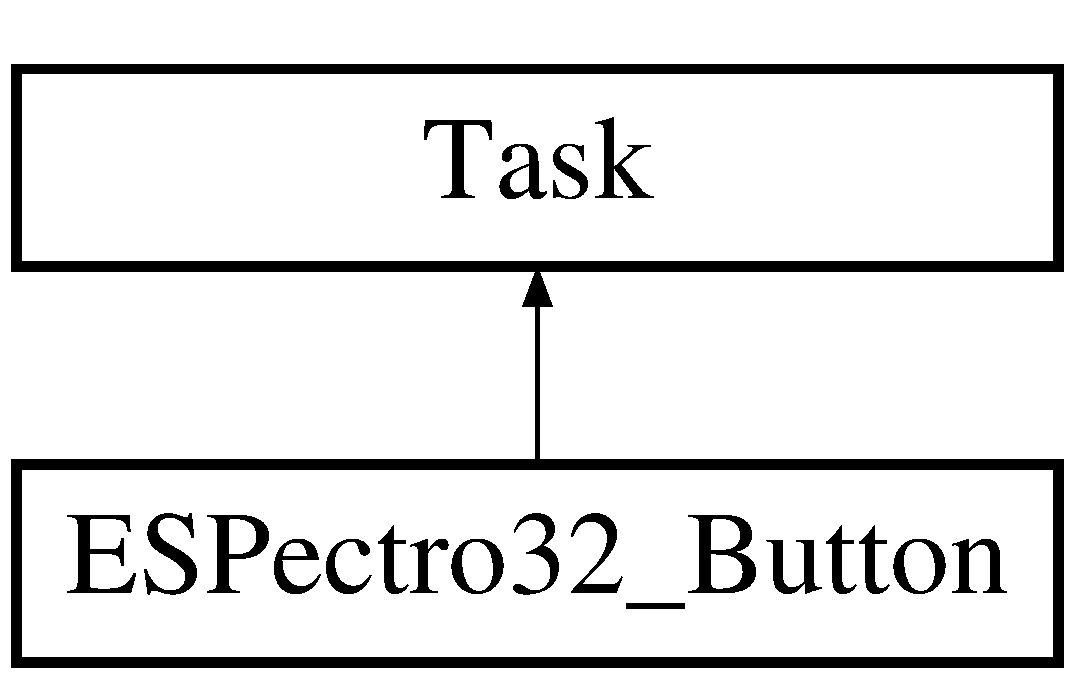
\includegraphics[height=2.000000cm]{classESPectro32__Button}
\end{center}
\end{figure}
\subsection*{Public Types}
\begin{DoxyCompactItemize}
\item 
enum {\bfseries Button\-\_\-\-State} \{ \\*
{\bfseries E\-S\-Pectro32\-Button\-Unknown} = 0, 
{\bfseries E\-S\-Pectro32\-Button\-Pressed}, 
{\bfseries E\-S\-Pectro32\-Button\-Released}, 
{\bfseries E\-S\-Pectro32\-Button\-Second\-Pressed}, 
\\*
{\bfseries E\-S\-Pectro32\-Button\-Waiting\-For\-Long\-Pressed}, 
{\bfseries E\-S\-Pectro32\-Button\-Long\-Pressed}
 \}
\item 
\hypertarget{classESPectro32__Button_afff4b934b4520b3c42d2792c67dbbe50}{typedef std\-::function$<$ void()$>$ {\bfseries Button\-Action\-Callback}}\label{classESPectro32__Button_afff4b934b4520b3c42d2792c67dbbe50}

\end{DoxyCompactItemize}
\subsection*{Public Member Functions}
\begin{DoxyCompactItemize}
\item 
\hypertarget{classESPectro32__Button_a0e823e4ff38fa5a16858d8a0267169ed}{{\bfseries E\-S\-Pectro32\-\_\-\-Button} (uint8\-\_\-t gpio, boolean active\-High=false)}\label{classESPectro32__Button_a0e823e4ff38fa5a16858d8a0267169ed}

\item 
\hypertarget{classESPectro32__Button_a7055a1c1acfa459a1c81bd0b08681159}{void \hyperlink{classESPectro32__Button_a7055a1c1acfa459a1c81bd0b08681159}{begin} ()}\label{classESPectro32__Button_a7055a1c1acfa459a1c81bd0b08681159}

\begin{DoxyCompactList}\small\item\em Must be called as soon as possible to do initialization stuffs. \end{DoxyCompactList}\item 
\hypertarget{classESPectro32__Button_a9af097046592195c0778b98ba50022eb}{void {\bfseries start} (void $\ast$task\-Data=nullptr)}\label{classESPectro32__Button_a9af097046592195c0778b98ba50022eb}

\item 
\hypertarget{classESPectro32__Button_a8706dbe3931f2e60de36a667e451ad2c}{Button\-\_\-\-State {\bfseries get\-State} ()}\label{classESPectro32__Button_a8706dbe3931f2e60de36a667e451ad2c}

\item 
\hypertarget{classESPectro32__Button_a62289ae77d95dbc54dfcadd84adb95a8}{void {\bfseries run} ()}\label{classESPectro32__Button_a62289ae77d95dbc54dfcadd84adb95a8}

\item 
\hypertarget{classESPectro32__Button_a7c07861f069f7af51a4a9e29b8bcdbdf}{void {\bfseries run\-Async} (void $\ast$data)}\label{classESPectro32__Button_a7c07861f069f7af51a4a9e29b8bcdbdf}

\item 
\hypertarget{classESPectro32__Button_a62b9b6106ef44eefd820ec79bcf410ed}{void {\bfseries on\-Button\-Down} (Button\-Action\-Callback cb)}\label{classESPectro32__Button_a62b9b6106ef44eefd820ec79bcf410ed}

\item 
\hypertarget{classESPectro32__Button_ab0d4b247a9964a4e0be84c7e1f820aaa}{void {\bfseries on\-Button\-Up} (Button\-Action\-Callback cb)}\label{classESPectro32__Button_ab0d4b247a9964a4e0be84c7e1f820aaa}

\item 
\hypertarget{classESPectro32__Button_a6c3d37c08d1ae0575417f6e9f0d7bd66}{void {\bfseries on\-Pressed} (Button\-Action\-Callback cb)}\label{classESPectro32__Button_a6c3d37c08d1ae0575417f6e9f0d7bd66}

\item 
\hypertarget{classESPectro32__Button_ad387123c630859eab0e0f85a8ede4679}{void {\bfseries on\-Long\-Pressed} (Button\-Action\-Callback cb)}\label{classESPectro32__Button_ad387123c630859eab0e0f85a8ede4679}

\item 
\hypertarget{classESPectro32__Button_aaa428fdecf890c9d2ca7ce9bd5d02b45}{void {\bfseries on\-Double\-Pressed} (Button\-Action\-Callback cb)}\label{classESPectro32__Button_aaa428fdecf890c9d2ca7ce9bd5d02b45}

\end{DoxyCompactItemize}


\subsection{Detailed Description}
E\-S\-Pectro32 button. 

This class is for working with button, especially attached button \char`\"{}\-A\char`\"{} and \char`\"{}\-B\char`\"{} on E\-S\-Pectro32. But nothing will stop you for working with external buttons.

Creating object\-: 
\begin{DoxyCode}
\hyperlink{classESPectro32__Button}{ESPectro32\_Button} buttonA(ESPECTRO32\_BUTTON\_A\_PIN);
\end{DoxyCode}


Attaching event handlers\-:


\begin{DoxyCode}
buttonA.onButtonUp([]() \{
    ESP\_LOGI(TAG, \textcolor{stringliteral}{"Button A up"});
\});
\end{DoxyCode}


That's for handling \char`\"{}on button up\char`\"{} event. 

The documentation for this class was generated from the following files\-:\begin{DoxyCompactItemize}
\item 
E\-S\-Pectro32\-\_\-\-Button.\-h\item 
E\-S\-Pectro32\-\_\-\-Button.\-cpp\end{DoxyCompactItemize}

\hypertarget{classESPectro32__LED}{\section{E\-S\-Pectro32\-\_\-\-L\-E\-D Class Reference}
\label{classESPectro32__LED}\index{E\-S\-Pectro32\-\_\-\-L\-E\-D@{E\-S\-Pectro32\-\_\-\-L\-E\-D}}
}
\subsection*{Public Member Functions}
\begin{DoxyCompactItemize}
\item 
\hypertarget{classESPectro32__LED_a2ec872a607f649dc20fa1a27e8748c6e}{{\bfseries E\-S\-Pectro32\-\_\-\-L\-E\-D} (uint8\-\_\-t pin=E\-S\-P\-E\-C\-T\-R\-O32\-\_\-\-L\-E\-D\-\_\-\-P\-I\-N, bool active\-High=false)}\label{classESPectro32__LED_a2ec872a607f649dc20fa1a27e8748c6e}

\item 
\hypertarget{classESPectro32__LED_ae400b1bf234437f37b399f89030522de}{void {\bfseries begin} ()}\label{classESPectro32__LED_ae400b1bf234437f37b399f89030522de}

\item 
\hypertarget{classESPectro32__LED_a68ceeb515c2884acc105675f52911f7f}{void {\bfseries turn\-On} ()}\label{classESPectro32__LED_a68ceeb515c2884acc105675f52911f7f}

\item 
\hypertarget{classESPectro32__LED_ad71509be67aae18c83ecc5af0dd27bc2}{void {\bfseries turn\-Off} ()}\label{classESPectro32__LED_ad71509be67aae18c83ecc5af0dd27bc2}

\item 
\hypertarget{classESPectro32__LED_a81487185442edd657d83a9fb57c1e698}{boolean {\bfseries is\-On} ()}\label{classESPectro32__LED_a81487185442edd657d83a9fb57c1e698}

\item 
\hypertarget{classESPectro32__LED_aa6aed07ae9a12dde1d9a86df99ad69a6}{byte {\bfseries get\-Pin} ()}\label{classESPectro32__LED_aa6aed07ae9a12dde1d9a86df99ad69a6}

\item 
\hypertarget{classESPectro32__LED_a05d65ff5cb4d266061e1b330fee25f77}{void {\bfseries toggle} ()}\label{classESPectro32__LED_a05d65ff5cb4d266061e1b330fee25f77}

\item 
\hypertarget{classESPectro32__LED_a8099ac834f4763b94d91849d96b001d6}{void {\bfseries blink} (uint32\-\_\-t interval=500, uint32\-\_\-t count=U\-I\-N\-T16\-\_\-\-M\-A\-X)}\label{classESPectro32__LED_a8099ac834f4763b94d91849d96b001d6}

\item 
\hypertarget{classESPectro32__LED_ae62a8f030848ec21aa3097120b2e9de0}{void {\bfseries fade} (uint32\-\_\-t duration=2000, uint32\-\_\-t count=U\-I\-N\-T16\-\_\-\-M\-A\-X)}\label{classESPectro32__LED_ae62a8f030848ec21aa3097120b2e9de0}

\item 
\hypertarget{classESPectro32__LED_a3398072d6b5e0969e7081db69baf2101}{void {\bfseries start\-Animation} ()}\label{classESPectro32__LED_a3398072d6b5e0969e7081db69baf2101}

\item 
\hypertarget{classESPectro32__LED_a30f73cf9358f05a725642f1e5e3bd884}{void {\bfseries stop\-Animation} ()}\label{classESPectro32__LED_a30f73cf9358f05a725642f1e5e3bd884}

\item 
\hypertarget{classESPectro32__LED_a93f2eebe2b745f8b5e4ad05d5833e80f}{bool {\bfseries is\-Animating} () const }\label{classESPectro32__LED_a93f2eebe2b745f8b5e4ad05d5833e80f}

\item 
\hypertarget{classESPectro32__LED_a7dc5619a2a6a47dafcd8ead44f0eba87}{void {\bfseries set\-Animation} (E\-S\-Pectro32\-\_\-\-L\-E\-D\-\_\-\-Animation\-Type anim\-Type, uint32\-\_\-t speed, uint32\-\_\-t count=U\-I\-N\-T16\-\_\-\-M\-A\-X)}\label{classESPectro32__LED_a7dc5619a2a6a47dafcd8ead44f0eba87}

\item 
\hypertarget{classESPectro32__LED_aaaedc9ff43ce728968e924aad46da54a}{void {\bfseries set\-Animation\-Timeout} (unsigned long time\-Out)}\label{classESPectro32__LED_aaaedc9ff43ce728968e924aad46da54a}

\end{DoxyCompactItemize}


The documentation for this class was generated from the following files\-:\begin{DoxyCompactItemize}
\item 
E\-S\-Pectro32\-\_\-\-L\-E\-D.\-h\item 
E\-S\-Pectro32\-\_\-\-L\-E\-D.\-cpp\end{DoxyCompactItemize}

\hypertarget{classESPectro32__LED__Animator}{\section{E\-S\-Pectro32\-\_\-\-L\-E\-D\-\_\-\-Animator Class Reference}
\label{classESPectro32__LED__Animator}\index{E\-S\-Pectro32\-\_\-\-L\-E\-D\-\_\-\-Animator@{E\-S\-Pectro32\-\_\-\-L\-E\-D\-\_\-\-Animator}}
}
Inheritance diagram for E\-S\-Pectro32\-\_\-\-L\-E\-D\-\_\-\-Animator\-:\begin{figure}[H]
\begin{center}
\leavevmode
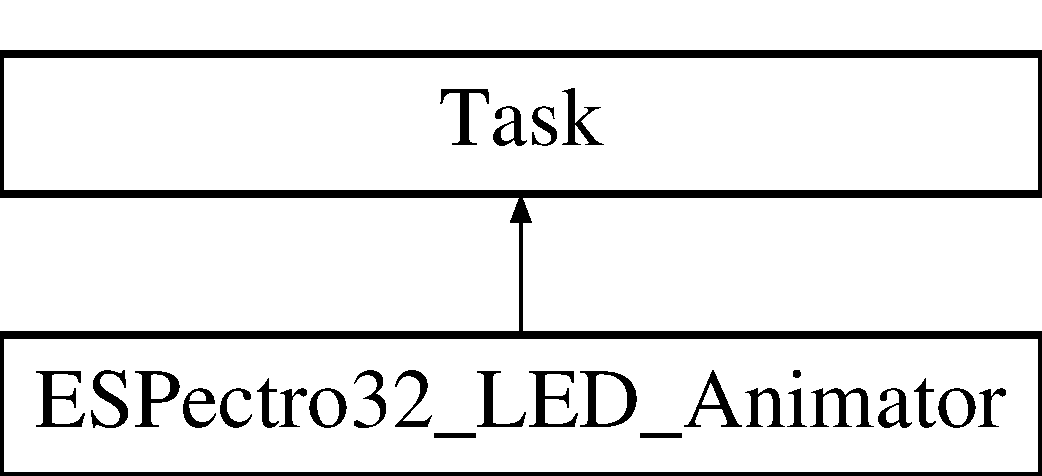
\includegraphics[height=2.000000cm]{classESPectro32__LED__Animator}
\end{center}
\end{figure}
\subsection*{Public Member Functions}
\begin{DoxyCompactItemize}
\item 
\hypertarget{classESPectro32__LED__Animator_a1dd78181b03d945041fdff57a77be3ba}{void {\bfseries init\-P\-W\-M} (byte pin, bool active\-High=false)}\label{classESPectro32__LED__Animator_a1dd78181b03d945041fdff57a77be3ba}

\item 
\hypertarget{classESPectro32__LED__Animator_a6ac0439b588360c898495b5a9922da13}{void {\bfseries set\-Animation} (E\-S\-Pectro32\-\_\-\-L\-E\-D\-\_\-\-Animation\-Type anim\-Type, uint32\-\_\-t speed)}\label{classESPectro32__LED__Animator_a6ac0439b588360c898495b5a9922da13}

\item 
\hypertarget{classESPectro32__LED__Animator_a4c6d8ac33ea56caf25989d9c0e4947a9}{bool {\bfseries run\-Animation} ()}\label{classESPectro32__LED__Animator_a4c6d8ac33ea56caf25989d9c0e4947a9}

\item 
\hypertarget{classESPectro32__LED__Animator_a3c1960b72ab66707137cfaca9dc1032d}{void {\bfseries set\-Brightness} (Rgb\-Led\-Color\-\_\-t max\-Out)}\label{classESPectro32__LED__Animator_a3c1960b72ab66707137cfaca9dc1032d}

\item 
void \hyperlink{classESPectro32__LED__Animator_acd696eea5a2982cf557706e9ea3ff0f6}{set\-Refresh\-Rate} (int refresh\-Rate)
\item 
\hypertarget{classESPectro32__LED__Animator_a4456c2b42e75121d256d856a6b482e72}{void {\bfseries run\-Async} (void $\ast$data)}\label{classESPectro32__LED__Animator_a4456c2b42e75121d256d856a6b482e72}

\item 
\hypertarget{classESPectro32__LED__Animator_a8f15c42dbd9232a36a841df15c624f56}{void {\bfseries start} ()}\label{classESPectro32__LED__Animator_a8f15c42dbd9232a36a841df15c624f56}

\item 
\hypertarget{classESPectro32__LED__Animator_aa82ac7f49d0ead5ed78a03b11e1a4d6d}{void {\bfseries stop} ()}\label{classESPectro32__LED__Animator_aa82ac7f49d0ead5ed78a03b11e1a4d6d}

\item 
\hypertarget{classESPectro32__LED__Animator_a98d875c4f6edffab25c18863237b5893}{void {\bfseries set\-Timeout} (unsigned long time\-Out)}\label{classESPectro32__LED__Animator_a98d875c4f6edffab25c18863237b5893}

\item 
\hypertarget{classESPectro32__LED__Animator_a1f5697a61b99a467a67091410e847d2e}{bool {\bfseries is\-Animating} ()}\label{classESPectro32__LED__Animator_a1f5697a61b99a467a67091410e847d2e}

\end{DoxyCompactItemize}


\subsection{Member Function Documentation}
\hypertarget{classESPectro32__LED__Animator_acd696eea5a2982cf557706e9ea3ff0f6}{\index{E\-S\-Pectro32\-\_\-\-L\-E\-D\-\_\-\-Animator@{E\-S\-Pectro32\-\_\-\-L\-E\-D\-\_\-\-Animator}!set\-Refresh\-Rate@{set\-Refresh\-Rate}}
\index{set\-Refresh\-Rate@{set\-Refresh\-Rate}!ESPectro32_LED_Animator@{E\-S\-Pectro32\-\_\-\-L\-E\-D\-\_\-\-Animator}}
\subsubsection[{set\-Refresh\-Rate}]{\setlength{\rightskip}{0pt plus 5cm}void E\-S\-Pectro32\-\_\-\-L\-E\-D\-\_\-\-Animator\-::set\-Refresh\-Rate (
\begin{DoxyParamCaption}
\item[{int}]{refresh\-Rate}
\end{DoxyParamCaption}
)}}\label{classESPectro32__LED__Animator_acd696eea5a2982cf557706e9ea3ff0f6}
Sets the maximum refresh rate in Hz (default value is 50 Hz). May be useful to reduce flickering in some cases. 

The documentation for this class was generated from the following files\-:\begin{DoxyCompactItemize}
\item 
E\-S\-Pectro32\-\_\-\-L\-E\-D.\-h\item 
E\-S\-Pectro32\-\_\-\-L\-E\-D.\-cpp\end{DoxyCompactItemize}

\hypertarget{classESPectro32__LedMatrix}{\section{E\-S\-Pectro32\-\_\-\-Led\-Matrix Class Reference}
\label{classESPectro32__LedMatrix}\index{E\-S\-Pectro32\-\_\-\-Led\-Matrix@{E\-S\-Pectro32\-\_\-\-Led\-Matrix}}
}
Inheritance diagram for E\-S\-Pectro32\-\_\-\-Led\-Matrix\-:\begin{figure}[H]
\begin{center}
\leavevmode
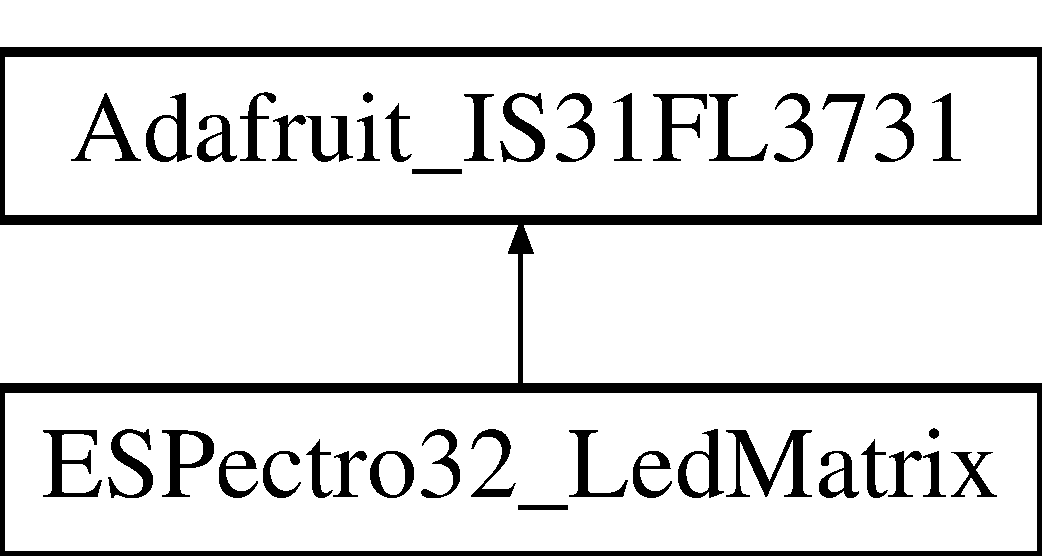
\includegraphics[height=2.000000cm]{classESPectro32__LedMatrix}
\end{center}
\end{figure}
\subsection*{Public Member Functions}
\begin{DoxyCompactItemize}
\item 
\hypertarget{classESPectro32__LedMatrix_acc508c724480c3a7a742e8cadfaa74ed}{void {\bfseries draw\-Pixel} (int16\-\_\-t x, int16\-\_\-t y, uint16\-\_\-t color)}\label{classESPectro32__LedMatrix_acc508c724480c3a7a742e8cadfaa74ed}

\end{DoxyCompactItemize}


The documentation for this class was generated from the following files\-:\begin{DoxyCompactItemize}
\item 
E\-S\-Pectro32\-\_\-\-Led\-Matrix.\-h\item 
E\-S\-Pectro32\-\_\-\-Led\-Matrix.\-cpp\end{DoxyCompactItemize}

\hypertarget{classESPectro32__RGBLED}{\section{E\-S\-Pectro32\-\_\-\-R\-G\-B\-L\-E\-D Class Reference}
\label{classESPectro32__RGBLED}\index{E\-S\-Pectro32\-\_\-\-R\-G\-B\-L\-E\-D@{E\-S\-Pectro32\-\_\-\-R\-G\-B\-L\-E\-D}}
}
Inheritance diagram for E\-S\-Pectro32\-\_\-\-R\-G\-B\-L\-E\-D\-:\begin{figure}[H]
\begin{center}
\leavevmode
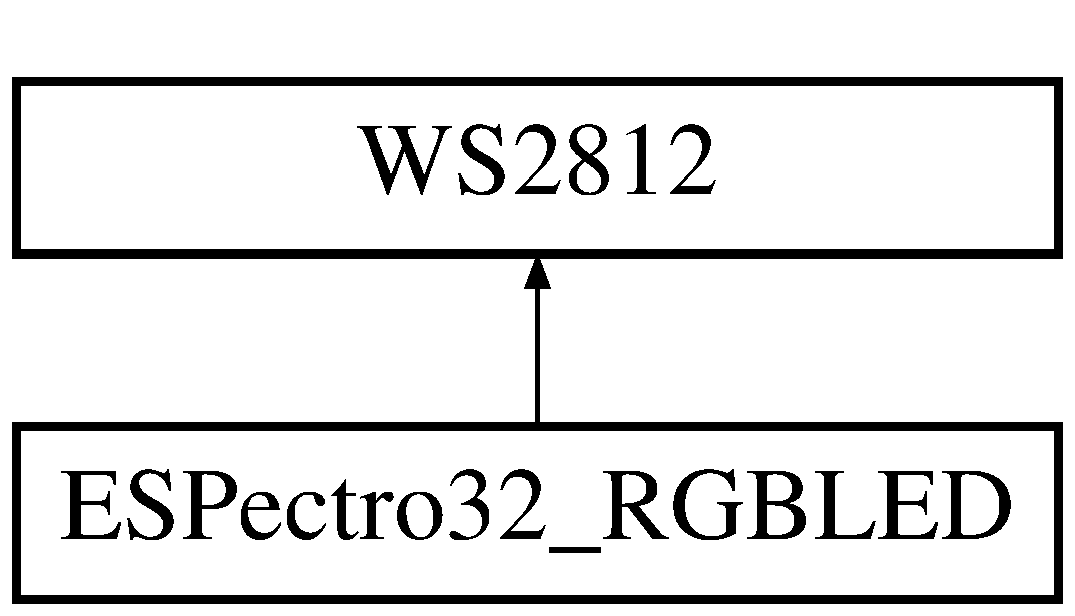
\includegraphics[height=2.000000cm]{classESPectro32__RGBLED}
\end{center}
\end{figure}
\subsection*{Public Member Functions}
\begin{DoxyCompactItemize}
\item 
\hypertarget{classESPectro32__RGBLED_a23fa473b601cc8cebd6a117285428c18}{{\bfseries E\-S\-Pectro32\-\_\-\-R\-G\-B\-L\-E\-D} (gpio\-\_\-num\-\_\-t gpio\-Num=E\-S\-P\-E\-C\-T\-R\-O32\-\_\-\-R\-G\-B\-L\-E\-D\-\_\-\-G\-P\-I\-O)}\label{classESPectro32__RGBLED_a23fa473b601cc8cebd6a117285428c18}

\end{DoxyCompactItemize}


The documentation for this class was generated from the following files\-:\begin{DoxyCompactItemize}
\item 
E\-S\-Pectro32\-\_\-\-R\-G\-B\-L\-E\-D.\-h\item 
E\-S\-Pectro32\-\_\-\-R\-G\-B\-L\-E\-D.\-cpp\end{DoxyCompactItemize}

\hypertarget{classESPectro32__RGBLED__Animation}{\section{E\-S\-Pectro32\-\_\-\-R\-G\-B\-L\-E\-D\-\_\-\-Animation Class Reference}
\label{classESPectro32__RGBLED__Animation}\index{E\-S\-Pectro32\-\_\-\-R\-G\-B\-L\-E\-D\-\_\-\-Animation@{E\-S\-Pectro32\-\_\-\-R\-G\-B\-L\-E\-D\-\_\-\-Animation}}
}


Base class of Neopixel R\-G\-B L\-E\-D animation. You should provide callback for anim\-Update\-Callback.  




{\ttfamily \#include $<$E\-S\-Pectro32\-\_\-\-R\-G\-B\-L\-E\-D\-\_\-\-Animation.\-h$>$}

Inheritance diagram for E\-S\-Pectro32\-\_\-\-R\-G\-B\-L\-E\-D\-\_\-\-Animation\-:\begin{figure}[H]
\begin{center}
\leavevmode
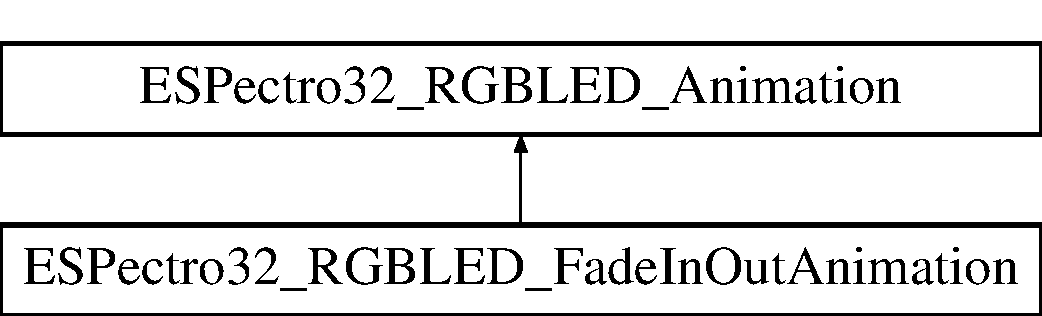
\includegraphics[height=2.000000cm]{classESPectro32__RGBLED__Animation}
\end{center}
\end{figure}
\subsection*{Public Member Functions}
\begin{DoxyCompactItemize}
\item 
\hypertarget{classESPectro32__RGBLED__Animation_adb4ace9959ddce9e4c4190bc8032bf77}{{\bfseries E\-S\-Pectro32\-\_\-\-R\-G\-B\-L\-E\-D\-\_\-\-Animation} (\hyperlink{classESPectro32__RGBLED}{E\-S\-Pectro32\-\_\-\-R\-G\-B\-L\-E\-D} \&rgb\-Led, Rgb\-Led\-Color\-\_\-t \&default\-Color)}\label{classESPectro32__RGBLED__Animation_adb4ace9959ddce9e4c4190bc8032bf77}

\item 
\hypertarget{classESPectro32__RGBLED__Animation_a8558246bd40b33eb7745428bdb5d009a}{void {\bfseries start} ()}\label{classESPectro32__RGBLED__Animation_a8558246bd40b33eb7745428bdb5d009a}

\item 
\hypertarget{classESPectro32__RGBLED__Animation_aef45fc6cc0054c980befc429fc25c90f}{void {\bfseries start} (W\-S2812\-Animator\-::\-Animation\-Update\-Callback anim\-Update\-Callback, W\-S2812\-Animator\-::\-Animation\-Finished\-Callback anim\-Finished\-Callback, uint16\-\_\-t duration=0, uint16\-\_\-t update\-Interval=0)}\label{classESPectro32__RGBLED__Animation_aef45fc6cc0054c980befc429fc25c90f}

\item 
\hypertarget{classESPectro32__RGBLED__Animation_a68276cca176858f56686f5a33c69f2d9}{void {\bfseries stop} ()}\label{classESPectro32__RGBLED__Animation_a68276cca176858f56686f5a33c69f2d9}

\item 
\hypertarget{classESPectro32__RGBLED__Animation_ae67369658f71b31b53229798bc6caa52}{void {\bfseries run} ()}\label{classESPectro32__RGBLED__Animation_ae67369658f71b31b53229798bc6caa52}

\item 
\hypertarget{classESPectro32__RGBLED__Animation_a2c8384a0665c0a7f356a05438e33b375}{void {\bfseries on\-Animation\-Completed} (W\-S2812\-Animator\-::\-Animation\-Finished\-Callback cb)}\label{classESPectro32__RGBLED__Animation_a2c8384a0665c0a7f356a05438e33b375}

\item 
\hypertarget{classESPectro32__RGBLED__Animation_abafab4b15281cea8b9127520c42ff194}{\hyperlink{classESPectro32__RGBLED}{E\-S\-Pectro32\-\_\-\-R\-G\-B\-L\-E\-D} \& {\bfseries Rgb\-Led} ()}\label{classESPectro32__RGBLED__Animation_abafab4b15281cea8b9127520c42ff194}

\end{DoxyCompactItemize}
\subsection*{Protected Member Functions}
\begin{DoxyCompactItemize}
\item 
\hypertarget{classESPectro32__RGBLED__Animation_a74b6ded71ed63e49f4c865258b5516ca}{W\-S2812\-Animator $\ast$ {\bfseries get\-Animator\-Ptr} ()}\label{classESPectro32__RGBLED__Animation_a74b6ded71ed63e49f4c865258b5516ca}

\end{DoxyCompactItemize}
\subsection*{Protected Attributes}
\begin{DoxyCompactItemize}
\item 
\hypertarget{classESPectro32__RGBLED__Animation_af280cb124d7a2ee7fa157625e49b816c}{\hyperlink{classESPectro32__RGBLED}{E\-S\-Pectro32\-\_\-\-R\-G\-B\-L\-E\-D} \& {\bfseries rgb\-Led\-\_\-}}\label{classESPectro32__RGBLED__Animation_af280cb124d7a2ee7fa157625e49b816c}

\item 
\hypertarget{classESPectro32__RGBLED__Animation_a89e7efa0cf8ca9c3353e2049e4316d39}{Rgb\-Led\-Color\-\_\-t \& {\bfseries default\-Color\-\_\-}}\label{classESPectro32__RGBLED__Animation_a89e7efa0cf8ca9c3353e2049e4316d39}

\item 
\hypertarget{classESPectro32__RGBLED__Animation_a33676837678e6e90c3eda53ba247d2e1}{W\-S2812\-Animator $\ast$ {\bfseries animator\-\_\-} = N\-U\-L\-L}\label{classESPectro32__RGBLED__Animation_a33676837678e6e90c3eda53ba247d2e1}

\item 
\hypertarget{classESPectro32__RGBLED__Animation_a442a1b2856cd5ac5b5f6081374aaea1e}{W\-S2812\-Animator\-::\-Animation\-Finished\-Callback {\bfseries anim\-Completed\-Cb\-\_\-} = N\-U\-L\-L}\label{classESPectro32__RGBLED__Animation_a442a1b2856cd5ac5b5f6081374aaea1e}

\item 
\hypertarget{classESPectro32__RGBLED__Animation_a5d33f43d0e6c27e9bc7f58171bde970b}{boolean {\bfseries animation\-Prev\-Started\-\_\-} = false}\label{classESPectro32__RGBLED__Animation_a5d33f43d0e6c27e9bc7f58171bde970b}

\item 
\hypertarget{classESPectro32__RGBLED__Animation_ae4c68e9d7db1fd7fe3c75b7502cb1cf2}{uint16\-\_\-t {\bfseries anim\-Completed\-Count\-\_\-} = 0}\label{classESPectro32__RGBLED__Animation_ae4c68e9d7db1fd7fe3c75b7502cb1cf2}

\item 
\hypertarget{classESPectro32__RGBLED__Animation_a519bddb3df7113d2014aaed34058fd29}{uint16\-\_\-t {\bfseries anim\-Max\-Count\-\_\-} = 0}\label{classESPectro32__RGBLED__Animation_a519bddb3df7113d2014aaed34058fd29}

\item 
\hypertarget{classESPectro32__RGBLED__Animation_a749e19362a0b3b359bd6a8681fee809e}{bool {\bfseries force\-Stop\-\_\-} = false}\label{classESPectro32__RGBLED__Animation_a749e19362a0b3b359bd6a8681fee809e}

\end{DoxyCompactItemize}


\subsection{Detailed Description}
Base class of Neopixel R\-G\-B L\-E\-D animation. You should provide callback for anim\-Update\-Callback. 

The documentation for this class was generated from the following files\-:\begin{DoxyCompactItemize}
\item 
E\-S\-Pectro32\-\_\-\-R\-G\-B\-L\-E\-D\-\_\-\-Animation.\-h\item 
E\-S\-Pectro32\-\_\-\-R\-G\-B\-L\-E\-D\-\_\-\-Animation.\-cpp\end{DoxyCompactItemize}

\hypertarget{classESPectro32__RGBLED__FadeInOutAnimation}{\section{E\-S\-Pectro32\-\_\-\-R\-G\-B\-L\-E\-D\-\_\-\-Fade\-In\-Out\-Animation Class Reference}
\label{classESPectro32__RGBLED__FadeInOutAnimation}\index{E\-S\-Pectro32\-\_\-\-R\-G\-B\-L\-E\-D\-\_\-\-Fade\-In\-Out\-Animation@{E\-S\-Pectro32\-\_\-\-R\-G\-B\-L\-E\-D\-\_\-\-Fade\-In\-Out\-Animation}}
}


A class of Neopixel R\-G\-B L\-E\-D fading in/out animation.  




{\ttfamily \#include $<$E\-S\-Pectro32\-\_\-\-R\-G\-B\-L\-E\-D\-\_\-\-Animation.\-h$>$}

Inheritance diagram for E\-S\-Pectro32\-\_\-\-R\-G\-B\-L\-E\-D\-\_\-\-Fade\-In\-Out\-Animation\-:\begin{figure}[H]
\begin{center}
\leavevmode
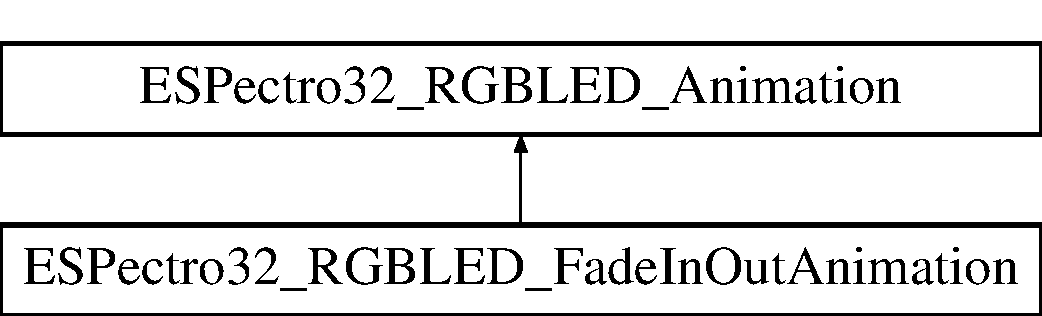
\includegraphics[height=2.000000cm]{classESPectro32__RGBLED__FadeInOutAnimation}
\end{center}
\end{figure}
\subsection*{Public Member Functions}
\begin{DoxyCompactItemize}
\item 
\hypertarget{classESPectro32__RGBLED__FadeInOutAnimation_aa60ab4ac0e9f8af2bba902f241b7893e}{{\bfseries E\-S\-Pectro32\-\_\-\-R\-G\-B\-L\-E\-D\-\_\-\-Fade\-In\-Out\-Animation} (\hyperlink{classESPectro32__RGBLED}{E\-S\-Pectro32\-\_\-\-R\-G\-B\-L\-E\-D} \&rgb\-Led, Rgb\-Led\-Color\-\_\-t \&default\-Color)}\label{classESPectro32__RGBLED__FadeInOutAnimation_aa60ab4ac0e9f8af2bba902f241b7893e}

\item 
void \hyperlink{classESPectro32__RGBLED__FadeInOutAnimation_a866667413ae40d902991884948a21215}{start} (uint16\-\_\-t duration=0, uint16\-\_\-t count=0)
\begin{DoxyCompactList}\small\item\em Start the animation. \end{DoxyCompactList}\item 
\hypertarget{classESPectro32__RGBLED__FadeInOutAnimation_a31c16b54569f6c2cac3586fcbb052c1d}{void {\bfseries stop} ()}\label{classESPectro32__RGBLED__FadeInOutAnimation_a31c16b54569f6c2cac3586fcbb052c1d}

\end{DoxyCompactItemize}
\subsection*{Additional Inherited Members}


\subsection{Detailed Description}
A class of Neopixel R\-G\-B L\-E\-D fading in/out animation. 

\subsection{Member Function Documentation}
\hypertarget{classESPectro32__RGBLED__FadeInOutAnimation_a866667413ae40d902991884948a21215}{\index{E\-S\-Pectro32\-\_\-\-R\-G\-B\-L\-E\-D\-\_\-\-Fade\-In\-Out\-Animation@{E\-S\-Pectro32\-\_\-\-R\-G\-B\-L\-E\-D\-\_\-\-Fade\-In\-Out\-Animation}!start@{start}}
\index{start@{start}!ESPectro32_RGBLED_FadeInOutAnimation@{E\-S\-Pectro32\-\_\-\-R\-G\-B\-L\-E\-D\-\_\-\-Fade\-In\-Out\-Animation}}
\subsubsection[{start}]{\setlength{\rightskip}{0pt plus 5cm}void E\-S\-Pectro32\-\_\-\-R\-G\-B\-L\-E\-D\-\_\-\-Fade\-In\-Out\-Animation\-::start (
\begin{DoxyParamCaption}
\item[{uint16\-\_\-t}]{duration = {\ttfamily 0}, }
\item[{uint16\-\_\-t}]{count = {\ttfamily 0}}
\end{DoxyParamCaption}
)}}\label{classESPectro32__RGBLED__FadeInOutAnimation_a866667413ae40d902991884948a21215}


Start the animation. 


\begin{DoxyParams}[1]{Parameters}
\mbox{\tt in}  & {\em duration} & How long in milisecond that one cycle of fading in and out takes place \\
\hline
\mbox{\tt in}  & {\em count} & How many cycle \\
\hline
\end{DoxyParams}


The documentation for this class was generated from the following files\-:\begin{DoxyCompactItemize}
\item 
E\-S\-Pectro32\-\_\-\-R\-G\-B\-L\-E\-D\-\_\-\-Animation.\-h\item 
E\-S\-Pectro32\-\_\-\-R\-G\-B\-L\-E\-D\-\_\-\-Animation.\-cpp\end{DoxyCompactItemize}

%--- End generated contents ---

% Index
\newpage
\phantomsection
\addcontentsline{toc}{chapter}{Index}
\printindex

\end{document}
